\graphicspath{{chapters/04/}}
\chapter{Tumor Evolution Studies via NGS data}
Tumor board: organism research oriented (and not) hospitals, patient not strictly assigned to one doctor but many specialist. E.g. oncologists, pathologists, geneticists... These boards are also a training asset for complex case studies and teach young doctors how to manege difficult events.
\\
\section{Tumor evolution}
%reference paper Tumour heterogeneity and resistance to cancer therapies
It is important to understand what are the somatic events that occur during tumor genesis/evolution and when they arise.\\
Cancer cells accumulate mutations due to both cell division and toxic agents (radiations, UV light,…); these mutations are maintained by the cell and lead to clonal expansion.  We can have a driver mutation kicking an oncogene or multiple mutations.
Typical traits of cancer are:
\begin{itemize}
\item Cancer is a dynamic disease, that's why evolution of the disease is so important to track.
\item During the course of disease, cancers generally become more heterogeneous, which is often related to treatment resistance.
\item The bulk tumor includes a diverse collection of cells harboring distinct molecular signatures with differential levels of sensitivity to treatment.
\item This heterogeneity might result in a non-uniform distribution of genetically distinct tumour-cell sub-populations across and within disease sites (spatial heterogeneity) or temporal variations in the molecular makeup of cancer cells (temporal heterogeneity).
\end{itemize}

\subsection{Tumor heterogeneity}
Every site of the genome with somatic mutations (point, inversion, …) is going to be differentially represented in tumor samples. Heterogeneity provides the fuel for resistance and is an obstacle to cancer treatment.
\\
Therefore, an accurate assessment of tumor heterogeneity is essential for the development of effective therapies. Emerging techniques to study with considerable potential to dissect the complex clonal architecture of cancers heterogeneity are: multi-region sequencing, single cell sequencing, analysis of autopsy samples, and longitudinal analysis of liquid biopsy samples.
\\
\\

However, techniques to study tumor heterogeneity are hindered by intra-patient heterogeneity, which divide into \textbf{spatial} and \textbf{temporal} heterogeneity.

\paragraph*{Spatial heterogeneity}
	The patient has several independent tumor masses, which share certain cells, but have a unique genetic makeup;

\paragraph*{Temporal heterogeneity}
	One mass changes content over time, naturally or under particular pressures.


\begin{figure}[H]
	\centering
	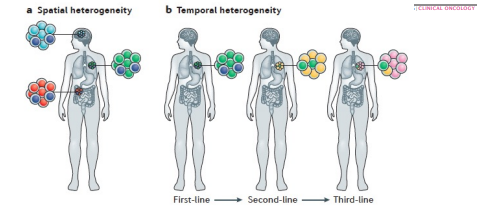
\includegraphics[width=0.7\textwidth]{heterogeneity.png}
	\caption{a) Spatial heterogeneity denotes an uneven distribution of cancer subclones across different regions of the primary tumor and/or metastatic sites. b) Temporal heterogeneity refers to variations in the molecular makeup of a single lesion over time, either as a result of natural progression of the tumor or as a result of exposure to selective pressures created by clinical interventions. Colors denote the presence of subclones with different genetic features.}
	\label{fig:hetero}
\end{figure}

\begin{figure}[H]
	\centering
	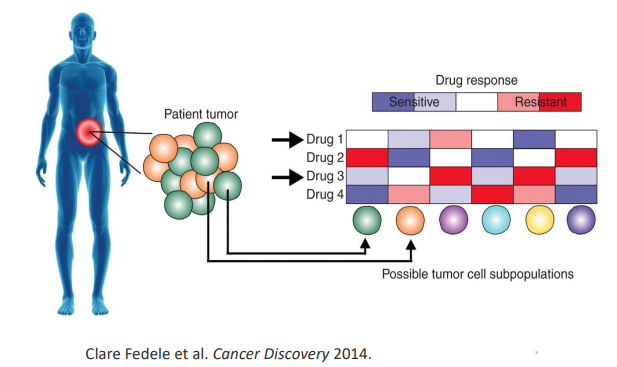
\includegraphics[width=0.6\textwidth]{treatment.png}
	\caption{x Certain cells of the tumor mass respond to treatment and some don't. Red = cell resistant to drug, blue = cell sensitive to drug. }
	\label{fig:hetero}
\end{figure}

\subsubsection{Linear an branching evolution}
It could be possible that some cells positively respond to treatment and others not, creating a heterogeneous population in the mass.
\\
The features of this set of cells changes over time. This evolution happens either because the new population \textbf{replaces} the older, or there's a \textbf{branching} and the tumor mass becomes heterogeneous.\\

\paragraph*{Linear evolution}
Sequential genetic alterations confer a fitness advantage such that successive generations are able to outcompete the preceding clones, which lack this fitness advantage. Surviving dominant clones harbor the ancestral mutation.

\paragraph*{Branch evolution}
Multiple genetically distinct populations can emerge from a common ancestral clone, with certain subclonal populations diverging from the common ancestor before others. The branching evolution is depicted in figure \ref{fig:branching}.

\begin{figure}[H]
	\centering
	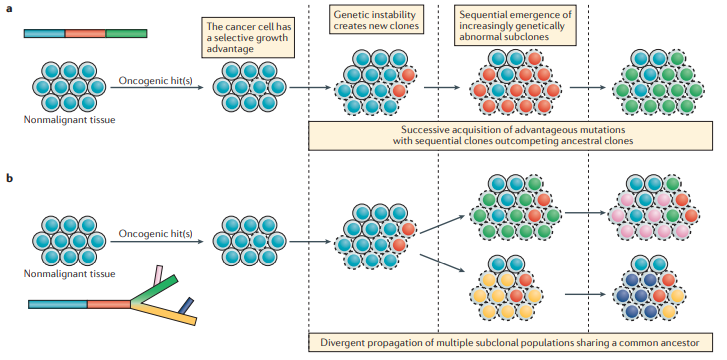
\includegraphics[width=0.7\textwidth]{branching.png}
	\caption{ a) everything branches out from the monoclonal origin, but b) polyclonal origin, independent metastatic processes. Cells from independent lesions meet and form a highly diverse metastatic tumor.}
	\label{fig:branching}
\end{figure}

How can we study tumor evolution? Example seen in class: prostate sample, multiple independent lesions. By browsing through the morphologies, we can find similarities for the expression of the same gene. Sanger sequencing can be used for very specific mutations. Through bulk DNA sequencing from each position, a representation of the tumor burden and features of all the different areas can be obtained.

\subsection{Treatment resistance}
How does resistance to treatment arise in cancer cells? Is treatment resistance encoded in the original cells or is it driven by the treatment itself?
\\
The two possibilities (also reported in figure \ref{fig:response}) are selection of clones that provide resistance, or transformation of clones under treatment pressure.

\paragraph*{Primary resistance}
Pre-existing heterogeneity fosters resistance. Only susceptible cells die and resistance cells continue dividing, allowing the tumor to regrow (high mass tumor).

\paragraph*{Acquired resistance}
Drug-tolerant, “persistent" cells generate resistant clones. At the time of diagnosis there are no markers, the de novo resistance alteration is developed afterward. Eventually, the resistant cells can from new tumors not responding to the drug.


\begin{figure}[H]
	\centering
	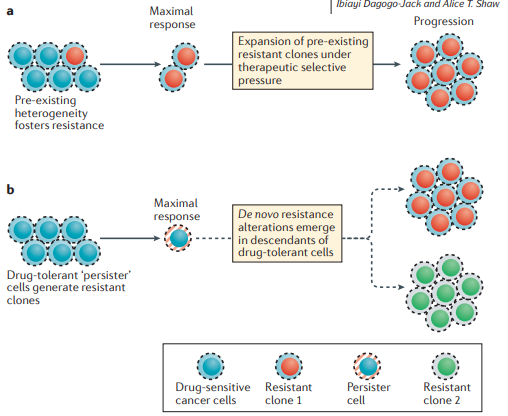
\includegraphics[width=0.7\textwidth]{response.png}
	\caption{ Tumor cells evolution driven by treatment.}
	\label{fig:response}
\end{figure}

\section{From sketches to sequencing data evolution information}
In order to study tumor evolution, we can use common and private lesions across multiple samples from the same individual to reconstruct the path.
Conversely, we can learn from multiple individuals at the same time points (select the most clonal lesion), with the goal of building a common clonal evolution map.
E.g. tumor suppressor gene NKX3-1 and PTEN lesions are shared between many individuals. Overall, in prostate cancer it is likely to have a subsequent PTEN mutation if CHD1 mutation is present.
\\
In general, we are interested into finding out which lesions occurred first and which is the model that fits better the data.

\subsection{Tumor evolution and heterogeneity}
To summarize, the difficult tasks one has to deal with when studying tumor data, and always need to study and take into account are:
\begin{multicols}{2}
\begin{itemize}
\item Intra tumor heterogeneity.
\item Inter tumor/intra patient heterogeneity.
\item Inter-patient heterogeneity.
\item Clinical/treatment relevance.
\item Time dependency.
\item Admixture DNA (tumor purity).
\end{itemize}
\end{multicols}

If properly investigated, they provide for insightful hints in the analysis.

\subsubsection{Admixture}
Whenever we take a piece of tissue from a patient, we have multiple cell types. The same happens with a biopsy, which will never be composed 100\% by cancer cells. This concept is referred to as \textbf{DNA admixture}.
\\
\textbf{Tumor purity} is computed as 1-DNA admixture. Purity is related to lesion aggressiveness (low purity is linked to less severity) and lesion classification (clonal or subclonal). In fact, every interpretation of somatic data needs to be interpreted in the context of tumor purity. Lesion is clonal if all tumor cells have it, a less present lesion instead might be subclonal.

%Deconvultion looking at NGS data. Lesion 100\% pure if the contamination of the adm of tumor cells is very low. \\

\section{Useful measures from NGS pipeline}
Also in this case we will be exploiting the polymorphic information that is present in the genetics of every individual. SNPs are very helpful in all somatic analysis.
\begin{itemize}
\item \textbf{Minor allele frequency, (MAF)}, frequency at which the alternative allele at a polymorphic site is represented in the population.
\item \textbf{Allelic fraction, (AF)}, how many times at a specific locus in a single individual we see the alternative base being represented. How many reads represent the alternative allele, how much support.
\end{itemize}

\subsection{Informative SNPs in cancer studies}
Informative SNPs are SNPs at which one individual has a heterozygous genotype; we can count allelic fraction and assess the proportion of reads supporting the alternative base.
If we have a deletion spanning a genomic area, at every informative SNP we will see that the allelic fraction, instead of being 50, will be either 0 or 100. Therefore, a diseased tissue will have an allelic distribution peaking at 0 or 1.
\\
\textit{Nref} is the percentage of reference base in the non-deleted allele.
\\
We can also track \textbf{beta ($\beta$)}, the percentage of neutral reads. If both alleles are equally represented, beta will be equal to 1.
Conversely, when only one allele is represented, beta is equal to 0.
How much beta is different from 1 is an indication of either admixture or subclonality of the lesion.
When only some cells in the sample are tumor cells, the distribution of AF will have two peaks.
\\
In each genomic segments that we are studying we many informative SNPs, at least two, to drive some conclusions. For example, figure \ref{fig:af_properties}.\\
How do we select informative SNPs? Use dbSNP database and select all heterozygous genotype sites, patient-centric analysis regardless of MAF. Obviously in the case of a target assay, it is possible to enrich for SNPs for high MAF, maximizing likelihood of finding informative SNPs (should be carefully designed).

\begin{figure}[H]
	\centering
	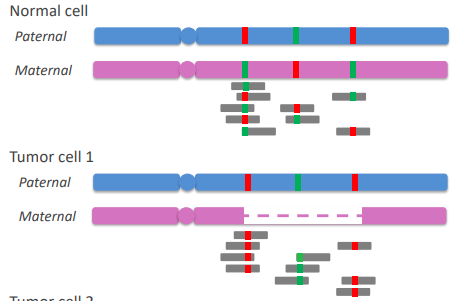
\includegraphics[width=0.5\textwidth]{af_properties.png}
	\caption{ Thanks to the presence of informative SNPs is very easy to detected the loss of an allele in the tumor cell.}
	\label{fig:af_properties}
\end{figure}

An example of the use of AF and beta measures for tumor data analysis in depicted in figure \ref{fig:a_b}.

\begin{figure}[htbp!]
	\centering
	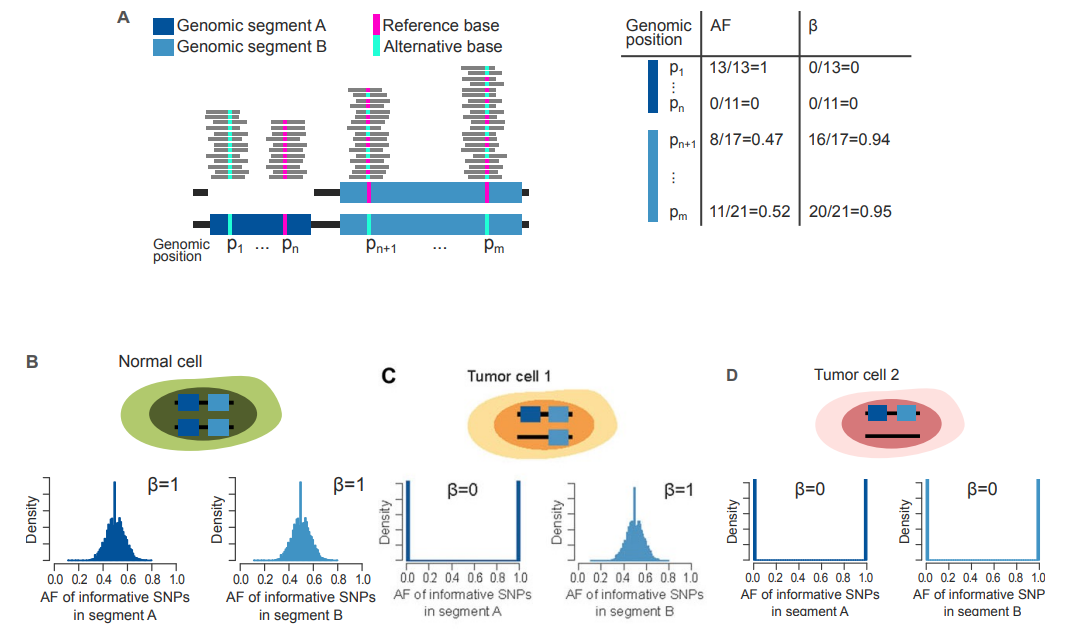
\includegraphics[width=0.8\textwidth]{a.png}
	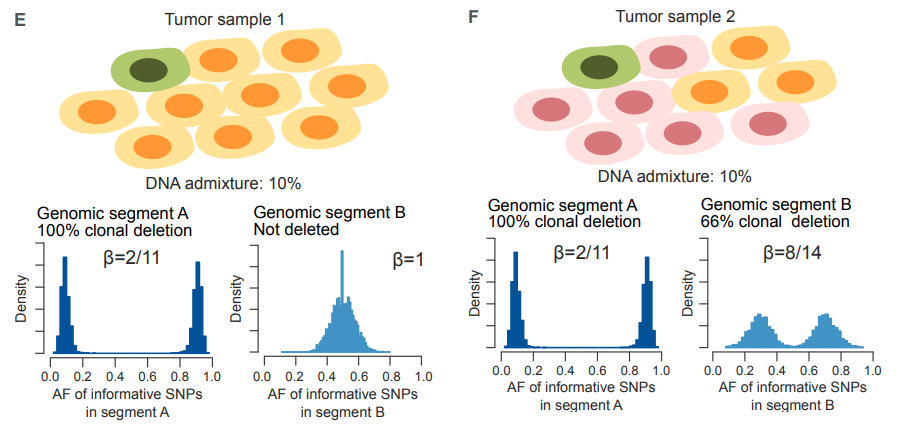
\includegraphics[width=0.8\textwidth]{b.png}
	\caption{
	\textbf{A)}Example of the allelic fraction (AF) and beta ($\beta$) in computed in five genomic positions ($p_1$ to $p_m$). Positions $p_1$ to $p_n$ are within a hemizygous deleted genomic segment A, while genomic positions $p_{n+1}$ to pm lie within a wild type genomic segment B.\\
\textbf{(B-D)} Examples of a normal cell and two different tumor cells. Tumor cells 1 and 2 differ for the status of genomic segment B. Histograms below cell cartoons report the expected distribution of the allelic fraction of SNPs in genomic segments A and B together with the associated beta values.\\
\textbf{(E-F)} Examples of two different tumor samples. Tumor sample 1 includes one normal cell and nine tumor cells with deleted genomic segment A and wild type genomic segment B. Tumor sample 2 differs from tumor sample 1 in the presence of six tumor cells with a hemizygous deletion of genomic segment B.
Expected distribution of the AF of informative SNPs together with estimated beta are depicted below each tumor sample cartoon.}
\label{fig:a_b}
\end{figure}

\subsection{Coverage and AF properties}
Does the mean coverage of the experiment impact on the ability to use the AF properties?\\
Intuitively, the deeper the sequencing the more likely it is to distinguish distribution that are not so close to each other. It is especially important when $\beta$ is close to zero. An example is shown in figure \ref{fig:beta}.


\begin{figure}[H]
	\centering
	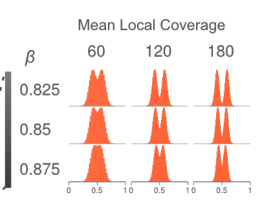
\includegraphics[width=0.4\textwidth]{beta.png}
	\caption{2X experiment: on average we have 2 reads per gene, very easy to miscall.\\
10X experiment: easy to do call, but in the case of tumor cells it becomes difficult. The higher the sequencing depth, the more accurate the calls will be (as it becomes easier to tell when a distribution has two peaks).
}
\label{fig:beta}
\end{figure}

\subsection{Computing Beta}
We can compute beta for each genomic segment S:
\begin{enumerate}
\item compute the observed distribution of the AF of informative SNPs in the genomic segment S;
\item find the values of Beta and Nref such that the expected distribution of the AF matches the observed AF;
\item compute uncertainty around Beta as a function of:
	\begin{enumerate}
	\item the mean coverage of S;
	\item the number of informative SNPs in S;
	\end{enumerate}
\end{enumerate}


\section{Global vs Local Estimates of admixture}\label{sec:admixture}
We'll discuss two types of sample and how to determine the differences in cell population (admixture).
\\
In sample one depicted in figure \ref{fig:sample1} there's a clonal cell population, meaning no heterogeneity. On the X axis we have genomic coordinates indexed by informative SNPs for that individual, on the Y axis the half AF.
\\
For all the informative SNPs present in this chunk of DNA, we see drops in AF that are smaller or wider, but more or less similar for each one of those lesions (drops). Meaning a drop or a gain in the amount of DNA that is almost identical in all of these chunks. \\
The representation of the lesions is supported by the same data along the stretch of DNA.
Thinking in terms of how much the AF distribution from 0 and 1 and the center is basically the same across all of them. Meaning, the level of admixture, both globally and locally, is the same. \\
Or, again, the amount of cells that have the first, second, third lesion etc. is the same.

\begin{figure}[H]
	\centering
	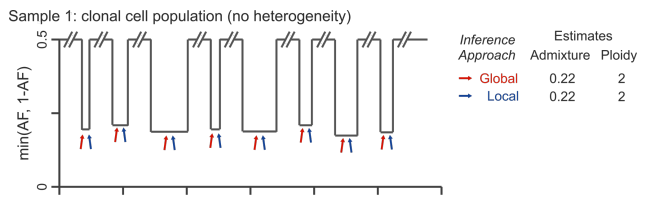
\includegraphics[width=0.7\textwidth]{sample1.png}
	\caption{In the clonal cell population how much the distribution deviates from AF is the same globally and locally.}
	\label{fig:sample1}
\end{figure}

In picture \ref{fig:sample2} below we can see another sample.
We can clearly discover multiclonal cell population. The depth of the lesion is proportional to the number of cells that carry the lesion.
In this case the definitions of local and global admixture change: a \textbf{global} value is a global value of tumor purity, a local value is a value of the clonality of the lesion in the diseased cell population.

\begin{figure}[H]
	\centering
	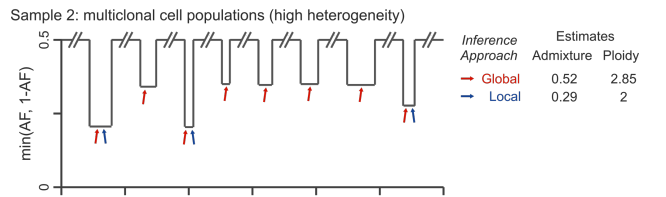
\includegraphics[width=0.7\textwidth]{sample2.png}
	\caption{We observe heterogeneity, the global and local values are different. A global value is relative to tumor purity, local to clonality. Admixture = 1-tumor purity}
	\label{fig:sample2}
\end{figure}

\subsubsection{Estimate of DNA admixture (1-Purity)}
We will now translate the concepts expressed in the previous sub-sections \ref{sec:admixture} in a 2-dimensional space, as shown in figure \ref{fig:2d}.

\begin{wrapfigure}{l}{0.5\textwidth}
	%\centering
	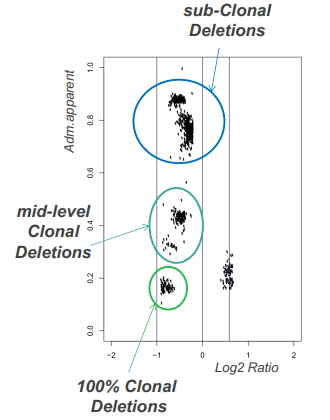
\includegraphics[width=0.7\linewidth]{adm.png}
	\caption{Multiple clusters, where each dot is a genomic segment. Lower clusters are used for the admixture, the others are subclonal.}
 \label{fig:2d}
\end{wrapfigure}

On the X axis we have the Log2 ratio measure and on the Y axis the admixture apparent, which is proportional to the beta  value.\\
The Log2 Ratio is basically tumor over normal in the log2 space. It allows to interpret info about every segment in the genome when coupled with the beta measure.
\\
The admixture apparent is calculated as

\begin{equation} \label{eq:adm}
\textit{Adm. apparent} = \frac{\beta}{2-\beta}
\end{equation}

This measure associates an apparent DNA admxiture to each monoallelic deletion. It is useful to calculate the clonality values, for which the formula is:

\begin{equation}
\textit{Clonality:} \frac{1 - \textit{Adm. apparent}}{1 - \textit{Adm. global}}
\end{equation}

The lowest cluster is the one used to assess admixture and the other ones are subclonal lesions.\\
Moreover, the closest the points are, the most probable it is that the lesions happened close in time, and viceversa.

\section{A challenging case (PR-2741*)}
Data of a real case of prostate cancer in which we can see a clear drop in coverage in region 2 of the 5th chromosome, while region 1 and 3 have equal coverage. The DNA present in region 2 could come either from admixing cells or from cells that do not have the deletion. \\
Looking at the AF of region 1, 2, 3, both from the tumor and the match normal normal sample we observe more or less the same two modes of distribution.\\
In the tumor sample in fact we do not see two peaks in 0 and 1 as expected. It could be signal of intervening normal cells, that bring the modes to the center, or subclonality event. \\


\begin{figure}
	\centering
	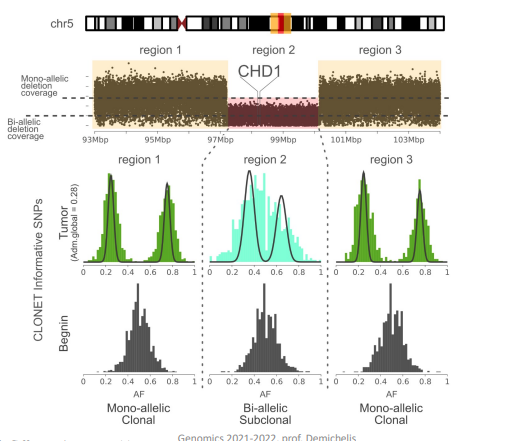
\includegraphics[width=0.7\linewidth]{PR_2741.png}
	\caption{ The distribution of heterozygous SNPs in benign cells is peaked in 0.5, while we observe two modes in tumor cells. The distance between the two modes is equal in 1 and 3, it’s proportional. In the middle we see that the two modes are moving towards the center, suggesting that the deletion is not likely 100\% clonal or it is clonal and shift is due to lack of deletion in 1 and 3. Subclonality: lesion with admixture}
	\label{fig:adm}
	\end{figure}
